%%%%%%%%%%%%%%%%%%%%%%%%%%%%%%%%%%%%%%%%%%%%%%%%%%%%%%%%%%%%%%%%%%%%%%
% How to use writeLaTeX: 
%
% You edit the source code here on the left, and the preview on the
% right shows you the result within a few seconds.
%
% Bookmark this page and share the URL with your co-authors. They can
% edit at the same time!
%
% You can upload figures, bibliographies, custom classes and
% styles using the files menu.
%
%%%%%%%%%%%%%%%%%%%%%%%%%%%%%%%%%%%%%%%%%%%%%%%%%%%%%%%%%%%%%%%%%%%%%%
\documentclass[12pt]{article}

\usepackage{sbc-template}

\usepackage{graphicx,url}
\usepackage{tabularx}
\usepackage{tikz}
\usetikzlibrary{arrows.meta}
\definecolor{procblue}{HTML}{dbe7f3}
\definecolor{procbluee}{HTML}{2f5c8a}
\definecolor{gengreen}{HTML}{e7f0e3}
\definecolor{gengreene}{HTML}{4a7a3a}
\definecolor{anlbeige}{HTML}{f6e9d8}
\definecolor{anlbeigee}{HTML}{9a6b2f}
\definecolor{outpurple}{HTML}{e9e2f0}
\definecolor{outpurplee}{HTML}{5e4a7a}

\usepackage{fvextra}
\DefineVerbatimEnvironment{MyVerbatim}{Verbatim}{
  breaklines=true,
  breakanywhere=true,
  breaksymbolleft={},
  breaksymbolright={},
  breakindent=0pt
}

%\usepackage[brazil]{babel}   
\usepackage[utf8]{inputenc}  

\sloppy

\title{Identificação e Análise de Vulnerabilidades em Código Gerado por IA: Uma Comparação entre Português e Inglês}

\author{Marcos Antônio Lommez Cândido Ribeiro\inst{1}, Matheus Alcântara Souza\inst{2} }

\address{
\hspace{-0.3cm}Depto. de Ciência da Computação -- Pontifícia Universidade Católica de Minas Gerais\\ Belo Horizonte -- MG -- Brasil\\
\vspace{-0.6cm}\hspace{-0.25cm}\email{tonilommez@hotmail.com,}
\vspace{-0.4cm}\hspace*{-0.25cm}\email{matheusalcantara@pucminas.br}
}

\begin{document} 

\maketitle

\begin{abstract}
The use of large language models (LLMs) for automatic code generation has become increasingly common in software development, providing significant productivity gains. However, the adoption of these tools in real-world environments raises concerns regarding the security of the generated code. In this context, this work investigates whether the natural language used in prompts, Portuguese or English, influences the incidence and types of vulnerabilities in AI-generated implementations. The analysis considers code generated across different programming languages and representative application scenarios, evaluated through static analysis tools and manual validation, with the goal of supporting a more informed and secure use of these technologies.
\end{abstract}
     
\begin{resumo}
O uso de modelos de linguagem de grande porte (LLMs) para geração automática de código tem se tornado cada vez mais comum no desenvolvimento de software, proporcionando ganhos significativos de produtividade. No entanto, a incorporação dessas ferramentas em ambientes reais levanta preocupações relacionadas à segurança do código gerado. Nesse contexto, este trabalho investiga se o idioma natural utilizado nos prompts, português ou inglês, influencia a incidência e o tipo de vulnerabilidades presentes nas implementações produzidas por modelos de IA. A análise considera códigos gerados em diferentes linguagens de programação e cenários representativos de aplicações reais, avaliados por meio de ferramentas de análise estática e validação manual, com o objetivo de apoiar uma utilização mais consciente e segura dessas tecnologias.
\end{resumo}

\section{Introdução}

A integração de modelos de linguagem de grande porte (LLMs) no desenvolvimento de software alterou significativamente a dinâmica de criação de código. Ferramentas como ChatGPT e Claude Code permitem que instruções em linguagem natural sejam convertidas diretamente em trechos funcionais, agilizando tarefas e reduzindo a carga cognitiva dos desenvolvedores. Contudo, à medida que esses sistemas são incorporados a ambientes de produção, surgem questionamentos sobre a confiabilidade e a segurança do código gerado \cite{pearce2021asleepkeyboardassessingsecurity}.

O problema central está no fato de que LLMs não são treinados para avaliar a qualidade de segurança das soluções que produzem. Esses modelos tendem a reproduzir padrões vulneráveis presentes nos dados de treinamento, muitas vezes oriundos de repositórios públicos \cite{dora2025hiddenrisksllmgeneratedweb}. Essa limitação torna frequentes falhas como injeções, exposição de credenciais e falta de validação de entrada. Além disso, há indícios de que o idioma natural utilizado nos \textit{prompts} influencia a consistência e a segurança das respostas. Modelos predominantemente treinados em inglês demonstram desempenho inferior em outros idiomas, produzindo saídas menos confiáveis ou ambíguas \cite{wang-etal-2024-languages}.

Diante disso, este trabalho propõe uma análise comparativa das vulnerabilidades em código gerado por modelos de IA a partir de prompts em português e inglês. O objetivo é identificar se o idioma natural exerce influência significativa sobre a incidência e o tipo de vulnerabilidade gerada, classificando as falhas segundo o \textit{Common Weakness Enumeration} (CWE) e comparando sua frequência relativa entre os dois contextos linguísticos.

Como contribuição, espera-se evidenciar o papel do idioma na segurança de código produzido por LLMs, oferecendo uma base empírica para orientar o uso responsável dessas ferramentas. O estudo também busca fortalecer o debate sobre práticas de auditoria e mitigação de riscos em geração automatizada de software.

O restante deste artigo está organizado da seguinte forma. A Seção~\ref{sec:revisao} apresenta a revisão de literatura e os trabalhos correlatos. A Seção~\ref{sec:metodologia} descreve a metodologia, incluindo os materiais, os programas-alvo, os procedimentos de análise e as implementações geradas. A Seção~\ref{sec:analise} detalha a análise de vulnerabilidades, abrangendo a análise estática e a revisão manual. A Seção~\ref{sec:resultados} discute os resultados obtidos. Por fim, a Seção~\ref{sec:conclusao} apresenta as conclusões e as direções para trabalhos futuros.

% ============================
\section{Revisão de Literatura}
\label{sec:revisao}

A geração de código assistida por inteligência artificial baseia-se em modelos de linguagem de grande porte que aprendem padrões sintáticos e estruturais a partir de grandes volumes de dados de texto e código. Embora capazes de produzir implementações funcionais, esses modelos não possuem mecanismos internos de validação de segurança, o que os torna propensos a replicar vulnerabilidades comuns. Estudos mostram que ferramentas como o GitHub Copilot geram códigos com falhas críticas de validação e autenticação, mesmo em tarefas simples \cite{pearce2021asleepkeyboardassessingsecurity}. De forma semelhante, o ChatGPT apresenta vulnerabilidades significativas em seus resultados, mesmo quando instruído explicitamente a produzir código seguro \cite{khoury2023securecodegeneratedchatgpt}.
  
Em comparação com o código humano, o código gerado por IA apresenta maior incidência de padrões inseguros e menor diversidade estrutural, o que o torna mais suscetível a ataques automatizados. Esses modelos tendem a negligenciar práticas seguras, expondo sistemas a fraquezas do tipo validação de entrada inadequada (CWE-20), injeção de SQL (CWE-89) e segredos embutidos no código (CWE-798) \cite{cotroneo2025humanwrittenvsaigeneratedcode}. Mesmo modelos mais recentes mantêm taxas elevadas de vulnerabilidade após ajustes em suas versões. Parte dessas deficiências está ligada à forma como os modelos aprendem com exemplos vulneráveis contidos nos repositórios públicos de onde extraem conhecimento \cite{dora2025hiddenrisksllmgeneratedweb}.

Além dos riscos diretos de segurança, há também fatores linguísticos e contextuais que afetam a robustez do código gerado. A qualidade das respostas fornecidas pelos modelos varia de acordo com o idioma do \textit{prompt}, já que a maior parte do treinamento é feita sobre dados em inglês \cite{wang-etal-2024-languages}. Em idiomas menos representados, observa-se redução na coerência sintática e na precisão semântica, o que pode comprometer instruções críticas relacionadas à segurança \cite{kumar2025polyguardmultilingualsafetymoderation}.

Benchmarks multilíngues recentes, como o CRUXEval-X, apontam que modelos de linguagem apresentam desempenho desigual em tarefas que envolvem raciocínio e execução de código em múltiplas linguagens \cite{xu2025cruxevalxbenchmarkmultilingualcode}. Esse fenômeno reforça a hipótese de que o idioma natural e o contexto linguístico de instrução podem exercer influência direta sobre a segurança do código produzido por IA. Além disso, estudos sobre vulnerabilidade em projetos multilíngues de software apontam que diferenças estruturais entre idiomas de programação aumentam a probabilidade de falhas, sugerindo que o contexto linguístico, tanto natural quanto técnico, impacta diretamente o comportamento de segurança \cite{10.1145/3540250.3549173}.

\subsection{Trabalhos Correlatos}

Diversos estudos têm investigado a segurança de código gerado por LLMs sob diferentes perspectivas. Um dos primeiros trabalhos sistemáticos avaliou o GitHub Copilot e identificou que cerca de 40\% das soluções geradas apresentavam vulnerabilidades conhecidas, especialmente falhas de validação e injeção de código \cite{pearce2021asleepkeyboardassessingsecurity}. Outro estudo concentrou-se no ChatGPT, revelando que mesmo instruções explícitas de segurança não impediram a geração de trechos inseguros, incluindo erros em autenticação e manipulação de dados sensíveis \cite{khoury2023securecodegeneratedchatgpt}.

Os estudos sobre segurança de código gerado por IA ampliaram o escopo de análise para diversas áreas, como aplicações web, mostrando que independentemente do tipo de aplicação, os modelos continuam propensos a falhas críticas relacionadas à autenticação, controle de sessão e sanitização de entradas \cite{dora2025hiddenrisksllmgeneratedweb}. Considerando também múltiplas linguagens de programação e diferentes contextos de uso, o desempenho e a consistência dos modelos variam dependendo da linguagem, refletindo limitações estruturais no entendimento semântico do código \cite{xu2025cruxevalxbenchmarkmultilingualcode}. Comparações entre código humano e IA-gerado indicam que a inteligência artificial reproduz vulnerabilidades de forma sistemática, refletindo os padrões inseguros presentes nos dados de treinamento \cite{cotroneo2025humanwrittenvsaigeneratedcode}.

Outros estudos propõem métodos de avaliação combinando funcionalidade e segurança, buscando métricas mais realistas para mensurar risco. Esses trabalhos evidenciam que mesmo quando o código passa em testes de execução, ele pode continuar vulnerável por não ter sido projetado com foco em segurança \cite{peng2025cwevaloutcomedrivenevaluationfunctionality, belozerov2025securecodingaicreation}. Em paralelo, análises multilíngues sugerem que o desempenho e a robustez variam de acordo com o idioma e o ecossistema de desenvolvimento, reforçando a importância de investigar o impacto da linguagem natural sobre a segurança \cite{kharma2025securityqualityllmgeneratedcode}.

Apesar do avanço das pesquisas, ainda há uma lacuna clara: nenhum dos trabalhos existentes comparou sistematicamente a segurança de códigos gerados em diferentes idiomas naturais. A Tabela~\ref{tab:correlatos} posiciona este estudo frente aos principais trabalhos correlatos, evidenciando que o idioma natural do prompt permanece como dimensão não investigada. Assim, este estudo busca preencher essa ausência ao examinar de forma empírica a influência do português e do inglês sobre a incidência de vulnerabilidades em código gerado por modelos de IA.

\begin{table}[ht]
\centering
\caption{Comparação metodológica entre os trabalhos correlatos e este estudo}
\label{tab:correlatos}
\small
\begin{tabularx}{\textwidth}{p{4.2cm}X}
\hline
\textbf{Artigo} & \textbf{Foco} \\
\hline
Asleep at the Keyboard? & Avalia vulnerabilidades em código gerado pelo GitHub Copilot em 89 cenários de alto risco. \\ \hline
How Secure is Code Generated by ChatGPT? & Avalia segurança de código gerado pelo ChatGPT em cinco linguagens via análise manual. \\ \hline
Hidden Risks of LLM-Generated Web App Code & Investiga riscos de segurança em código de aplicações web gerado por múltiplos LLMs. \\ \hline
Human-Written vs.\ AI-Generated Code & Compara vulnerabilidades entre código humano e código gerado por IA em larga escala. \\ \hline
CRUXEval-X & Benchmark para raciocínio e execução de código em múltiplas linguagens por LLMs. \\ \hline
Security and Quality in LLM-Generated Code & Analisa segurança e qualidade de código LLM-gerado em múltiplos modelos e linguagens. \\ \hline
\textbf{Este trabalho} & \textbf{Compara o perfil de vulnerabilidades em código gerado a partir de prompts em português e inglês.} \\ \hline
\end{tabularx}
\end{table}


\section{Metodologia}
\label{sec:metodologia}

Para a execução do estudo, foram definidas métricas, condições experimentais e ferramentas de análise. O fluxo experimental seguiu as seguintes etapas: elaboração dos prompts equivalentes em PT-BR e EN-US para cada cenário; geração do código pelos dois modelos selecionados; obtenção das implementações independentes; aplicação da análise estática e da revisão manual de segurança; classificação das vulnerabilidades por CWE e severidade; e, por fim, consolidação e comparação dos resultados por idioma, modelo e linguagem de programação. A Figura~\ref{fig:metodologia-consolidada} sintetiza esse encadeamento, incorporando tanto a composição das implementações quanto as etapas de avaliação adotadas no estudo.

\begin{figure}[ht]
\centering
\resizebox{0.78\linewidth}{!}{%
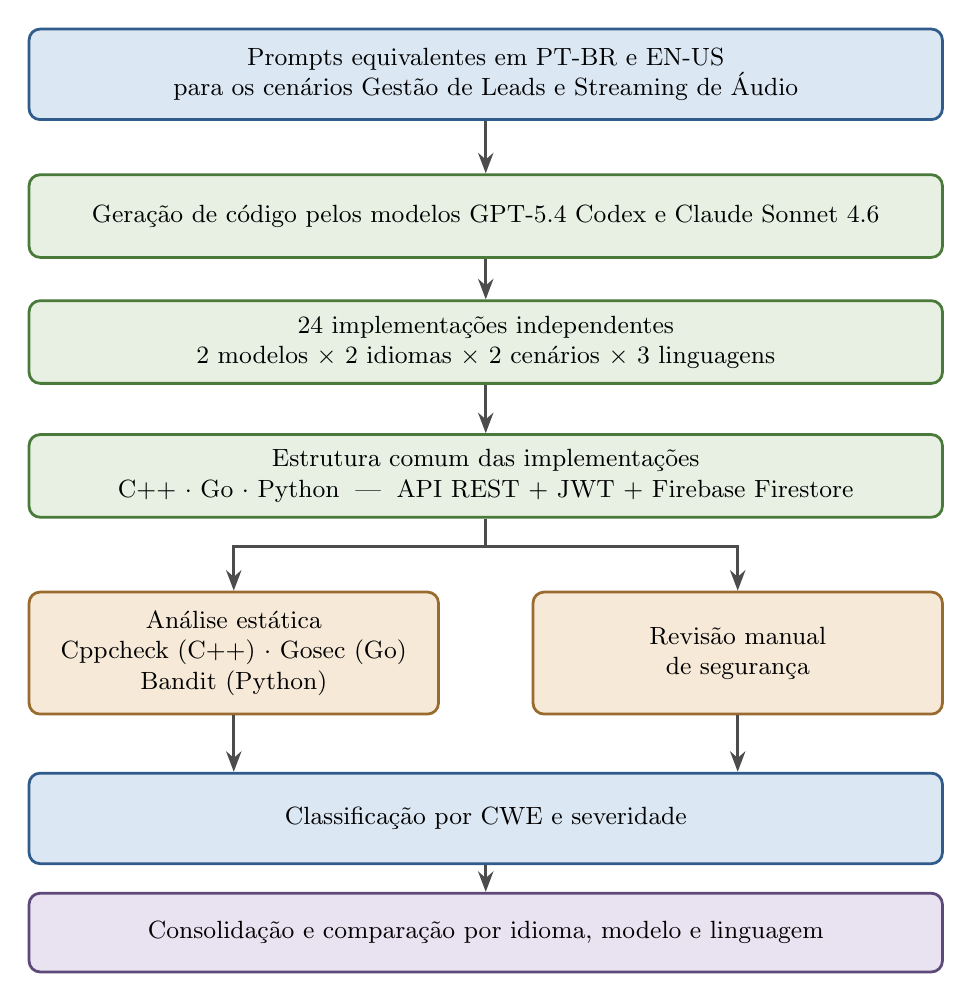
\begin{tikzpicture}[
    font=\small,
    proc/.style={rectangle, rounded corners=4pt, draw=procbluee, fill=procblue, line width=1pt, minimum width=11.6cm, minimum height=1.15cm, align=center, inner sep=5pt},
    gen/.style={rectangle, rounded corners=4pt, draw=gengreene, fill=gengreen, line width=1pt, minimum width=11.6cm, minimum height=1.05cm, align=center, inner sep=5pt},
    anl/.style={rectangle, rounded corners=4pt, draw=anlbeigee, fill=anlbeige, line width=1pt, minimum width=5.2cm, minimum height=1.55cm, align=center, inner sep=5pt},
    result/.style={rectangle, rounded corners=4pt, draw=outpurplee, fill=outpurple, line width=1pt, minimum width=11.6cm, minimum height=1.0cm, align=center, inner sep=5pt},
    fl/.style={-{Stealth[length=2.6mm]}, line width=1.0pt, draw=black!70}
  ]
  \node[proc] (p1) at (0, 8.9) {Prompts equivalentes em PT-BR e EN-US\\para os cenários Gestão de Leads e Streaming de Áudio};
  \node[gen]  (p2) at (0, 7.1) {Geração de código pelos modelos GPT-5.4 Codex e Claude Sonnet 4.6};
  \node[gen]  (p3) at (0, 5.5) {24 implementações independentes\\2 modelos $\times$ 2 idiomas $\times$ 2 cenários $\times$ 3 linguagens};
  \node[gen]  (p4) at (0, 3.8) {Estrutura comum das implementações\\C++ $\cdot$ Go $\cdot$ Python \;|\; API REST + JWT + Firebase Firestore};

  \node[anl]  (p5) at (-3.2, 1.55) {Análise estática\\Cppcheck (C++) $\cdot$ Gosec (Go)\\Bandit (Python)};
  \node[anl]  (p6) at ( 3.2, 1.55) {Revisão manual\\de segurança};

  \node[proc] (p7) at (0, -0.55) {Classificação por CWE e severidade};
  \node[result]  (p8) at (0, -2.0) {Consolidação e comparação por idioma, modelo e linguagem};

  \draw[fl] (p1) -- (p2);
  \draw[fl] (p2) -- (p3);
  \draw[fl] (p3) -- (p4);
  \draw[fl] (p4.south) -- ++(0,-0.35) -| (p5.north);
  \draw[fl] (p4.south) -- ++(0,-0.35) -| (p6.north);
  \draw[fl] (p5.south) -- (p5.south |- p7.north);
  \draw[fl] (p6.south) -- (p6.south |- p7.north);
  \draw[fl] (p7.south) -- (p8.north);
\end{tikzpicture}%
}
\caption{Fluxo metodológico consolidado do estudo, incluindo a geração das implementações, sua estrutura comum e as etapas de análise}
\label{fig:metodologia-consolidada}
\end{figure}

\subsection{Materiais e Configuração Experimental}

A análise contemplou três linguagens de programação que representam diferentes níveis de abstração, considerando que esse fator possivelmente afeta a probabilidade e o tipo de vulnerabilidades surgidas em implementações automáticas: C++ (baixo nível), Go (nível intermediário) e Python (alto nível).

A geração de código foi realizada por dois modelos comerciais populares durante o período de desenvolvimento: GPT-5.4 Codex, da OpenAI, e Claude Sonnet 4.6, da Anthropic. O acesso foi efetuado via aplicação desktop e todas as chamadas foram registradas com identificação de versão e idioma do prompt. A detecção de vulnerabilidades combinou análise estática com verificadores específicos de cada linguagem: Cppcheck 2.18.0 para C++, Gosec para Go e Bandit 1.9.4 para Python.

\subsection{Programas-alvo}

Os experimentos contemplaram dois cenários representativos de aplicações reais. O primeiro, denominado Gestão de Leads, consiste em um serviço REST com autenticação JWT, CRUD completo de leads, importação e exportação via CSV/Excel, dashboard e frontend desktop-first. O segundo, Streaming de Áudio, é um serviço de upload e reprodução de músicas com autenticação JWT, cadastro de artistas, gerenciamento de catálogo e streaming de arquivos de áudio. Cada cenário foi solicitado aos modelos em versões equivalentes dos prompts em PT-BR e EN-US. Combinando-se os dois modelos, os dois idiomas, os dois cenários e as três linguagens selecionadas, obteve-se um conjunto de 24 implementações independentes.

\subsection{Procedimentos de Análise}

Para cada cenário foi elaborado um prompt contendo descrição do contexto, requisitos, entradas e saídas esperadas e o ambiente alvo, produzido em PT-BR e EN-US e enviado a cada modelo. Foi aceita a primeira resposta gerada, sem solicitar regeneração, de modo a capturar o comportamento padrão do modelo em resposta a um único input, simulando um uso indiscriminado e não supervisionado. Prompts adicionais foram utilizados apenas quando o código gerado não compilava ou estava incompleto.

Cada artefato produzido foi submetido às ferramentas de análise estática correspondentes, obtendo-se relatórios com regra violada, descrição, localização, severidade e mapeamento para CWE quando disponível. Em seguida, as vulnerabilidades identificadas foram classificadas conforme o Common Weakness Enumeration (CWE), registrando-se modelo, idioma, linguagem de programação, cenário, trecho afetado e severidade final. Os dados consolidados foram então agregados por modelo, idioma e linguagem, calculando-se diferenças percentuais e taxas de ocorrência para identificação de padrões.

% ============================
\subsection{Implementações}

As implementações e os artefatos auxiliares da análise foram organizados em repositório público para fins de reprodutibilidade\footnote{\url{https://github.com/ToniLommez/tcc-seguranca-codigo-ia}}. Em todos os casos, os sistemas gerados apresentaram uma estrutura funcional comum, com backend em API REST, autenticação via JWT e integração com Firebase Firestore. Essa organização experimental, bem como o encadeamento entre geração, análise estática e revisão manual, encontra-se sintetizada na Figura~\ref{fig:metodologia-consolidada}. Exemplos dos prompts utilizados em português e inglês são apresentados nos Apêndices~\ref{apendice:prompt-pt} e~\ref{apendice:prompt-en}.

% ============================
\section{Análise de Vulnerabilidades}
\label{sec:analise}

A avaliação de segurança das implementações combinou duas abordagens complementares. A análise estática examina o código-fonte sem executá-lo, por meio de ferramentas automatizadas que percorrem a estrutura do programa em busca de padrões reconhecidamente inseguros; é rápida e reprodutível, porém limitada ao conjunto de regras de cada ferramenta. A revisão manual consiste na leitura e interpretação do código-fonte com base em conhecimento e experiência em segurança, capaz de identificar falhas de lógica, autorização e configuração que escapam às heurísticas automatizadas, ao custo de maior esforço.

Não foi empregada análise dinâmica neste estudo, por se tratar de uma abordagem que demandaria um escopo distinto de pesquisa, com maior complexidade na definição, configuração e controle dos ambientes de execução gerados. Assim, optou-se por delimitar o trabalho à análise estática e à revisão manual, considerando-as suficientes para os objetivos comparativos propostos, ficando a análise dinâmica como possibilidade para investigações futuras.

\subsection{Análise Estática}

As 24 implementações foram submetidas às ferramentas de análise estática correspondentes à linguagem utilizada. A Tabela~\ref{tab:static} consolida o total de ocorrências reportadas por cada grupo.

\begin{table}[ht]
\centering
\caption{Ocorrências na análise estática por linguagem, modelo e idioma do prompt}
\label{tab:static}
\begin{tabular}{llrr}
\hline
\textbf{Linguagem} & \textbf{Modelo} & \textbf{PT-BR} & \textbf{EN-US} \\
\hline
C++ (Cppcheck) & Claude & 11 & 9 \\
C++ (Cppcheck) & GPT   & 5  & 10 \\
Go (Gosec)     & Claude & 21 & 36 \\
Go (Gosec)     & GPT   & 9  & 10 \\
Python (Bandit) & Claude & 4 & 4  \\
Python (Bandit) & GPT   & 2  & 0  \\
\hline
\textbf{Total}  &       & \textbf{52} & \textbf{69} \\
\hline
\end{tabular}
\end{table}

O Gosec apresentou sensibilidade consideravelmente maior que Cppcheck e Bandit, reportando em média mais ocorrências por projeto. Isso se deve à natureza das verificações: o Gosec analisa padrões de uso de API e configurações de segurança em Go, como cookies sem atributo \texttt{Secure} e XSS por análise de fluxo, enquanto o Cppcheck foca predominantemente em qualidade de código e o Bandit detecta padrões específicos em Python. O Claude gerou significativamente mais ocorrências estáticas (85) que o GPT (36), resultado influenciado principalmente pelos projetos Go, onde o Claude produziu implementações com maior número de chamadas de API sujeitas a verificações do Gosec. Em relação ao idioma, projetos gerados a partir de prompts em EN-US acumularam mais ocorrências (69) que os em PT-BR (52), diferença concentrada nos projetos Go do Claude. Os totais das duas abordagens são comparáveis em volume (121 ocorrências na análise estática e 115 na revisão manual), embora cubram conjuntos distintos de vulnerabilidades: a análise estática detecta automaticamente padrões formalizados no código, enquanto a revisão manual identifica falhas de lógica, autorização e configuração que escapam às heurísticas das ferramentas.

% ============================
\subsection{Revisão Manual de Segurança}

Complementando a análise estática, foi realizada uma revisão manual de segurança de cada uma das 24 implementações, com leitura e análise de todos os arquivos de código-fonte de forma independente, sem consulta prévia aos relatórios de análise estática ou a revisões de outros projetos, evitando assim viés na identificação de vulnerabilidades. Foram inspecionados aspectos como gestão de credenciais e segredos, configuração de autenticação e autorização, exposição de dados sensíveis, validação de entradas, políticas de CORS e cabeçalhos de segurança, transmissão de tokens, configuração de TLS e padrões de uso de criptografia. As vulnerabilidades identificadas foram classificadas conforme o CWE e categorizadas por severidade (Crítica, Alta, Média e Baixa), seguindo critérios alinhados ao OWASP.

A Tabela~\ref{tab:manual} apresenta o total de vulnerabilidades identificadas por grupo.

\begin{table}[ht]
\centering
\caption{Vulnerabilidades identificadas na revisão manual por linguagem, modelo e idioma}
\label{tab:manual}
\begin{tabular}{llrrr}
\hline
\textbf{Linguagem} & \textbf{Modelo} & \textbf{PT-BR} & \textbf{EN-US} & \textbf{Total} \\
\hline
C++ & Claude & 13 & 10 & 23 \\
C++ & GPT   & 10 & 11 & 21 \\
Go  & Claude &  9 & 10 & 19 \\
Go  & GPT   &  8 &  9 & 17 \\
Python & Claude &  8 & 11 & 19 \\
Python & GPT   &  8 &  8 & 16 \\
\hline
\textbf{Total} & & \textbf{56} & \textbf{59} & \textbf{115} \\
\hline
\end{tabular}
\end{table}

% ============================
\section{Resultados e Discussão}
\label{sec:resultados}

\subsection{Comparativo por Idioma do Prompt}

O total de vulnerabilidades identificadas nos projetos gerados a partir de prompts em PT-BR foi de 56, contra 59 nos projetos em EN-US, uma diferença de 5,4\%. A Figura~\ref{fig:comparativo} ilustra esta distribuição por linguagem de programação.

\begin{figure}[ht]
\centering
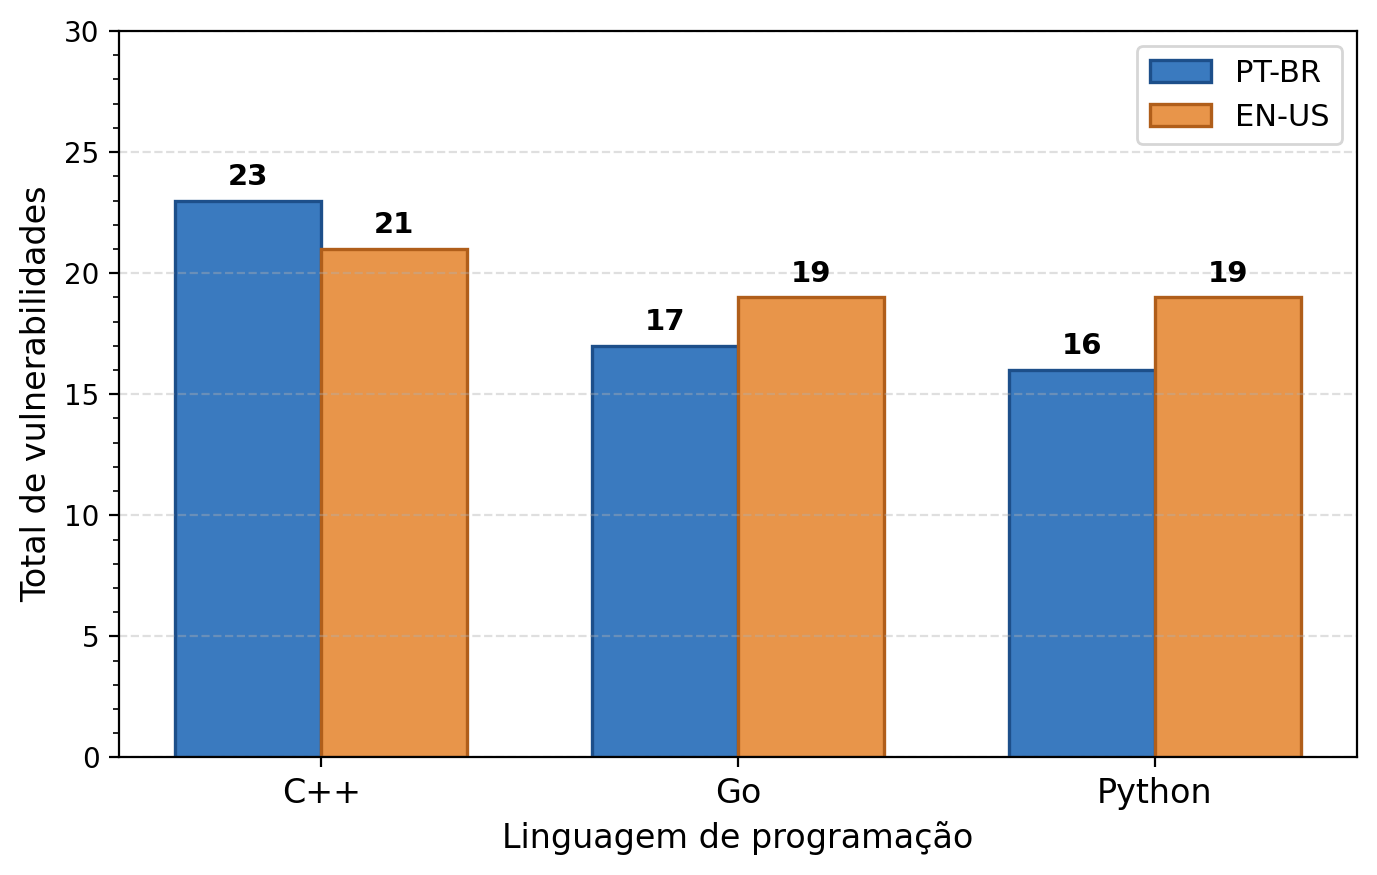
\includegraphics[width=0.85\textwidth]{comparativo_vulnerabilidades_idioma.png}
\caption{Distribuição de vulnerabilidades por linguagem de programação e idioma do prompt}
\label{fig:comparativo}
\end{figure}


A diferença observada é pequena e não apresenta um padrão consistente entre linguagens: em C++ o PT-BR gerou mais vulnerabilidades, enquanto em Go e Python o EN-US superou o PT-BR. A diferença não é suficiente para concluir que um idioma produz código significativamente mais seguro. Uma possível explicação é que os domínios de vulnerabilidade mais críticos, como ausência de TLS e credenciais embutidas, são independentes do idioma e refletem limitações sistêmicas dos modelos.

\subsection{Comparativo por Modelo}

O código gerado pelo Claude Sonnet 4.6 acumulou 61 vulnerabilidades no total, contra 54 do GPT-5.4 Codex, diferença de 12,9\%. Essa variação pode refletir diferenças na forma como cada modelo estrutura as implementações: o Claude tendeu a gerar projetos mais completos e com mais funcionalidades, o que naturalmente amplia a superfície de ataque.

\subsection{Média de Vulnerabilidades por Projeto}

A Tabela~\ref{tab:resumo} sumariza os totais e médias por dimensão de análise. Considerando as 24 implementações, a média geral foi de 4,8 vulnerabilidades por projeto. A variação entre idiomas é pequena (PT-BR: 4,7; EN-US: 4,9), enquanto a variação entre modelos é mais expressiva (Claude: 5,1; GPT: 4,5). O fator com maior impacto na média é a linguagem de programação: C++ apresenta média de 5,5 vulnerabilidades por projeto, contra 4,5 em Go e 4,4 em Python.

\begin{table}[ht]
\centering
\caption{Resumo comparativo de vulnerabilidades por dimensão}
\label{tab:resumo}
\begin{tabular}{llrrr}
\hline
\textbf{Dimensão} & \textbf{Grupo} & \textbf{Total} & \textbf{Média/projeto} & \textbf{\%} \\
\hline
Idioma  & PT-BR    & 56 & 4,7 & 48,7\% \\
        & EN-US    & 59 & 4,9 & 51,3\% \\
\hline
Modelo  & Claude   & 61 & 5,1 & 53,0\% \\
        & GPT      & 54 & 4,5 & 47,0\% \\
\hline
Linguagem & C++    & 44 & 5,5 & 38,3\% \\
          & Go     & 36 & 4,5 & 31,3\% \\
          & Python & 35 & 4,4 & 30,4\% \\
\hline
\textbf{Total} & & \textbf{115} & \textbf{4,8} & \\
\hline
\end{tabular}
\end{table}

O resultado de C++ com a maior média é consistente com a hipótese de que linguagens de menor abstração expõem o modelo a um conjunto maior de responsabilidades de segurança: gerenciamento manual de memória, configuração explícita de TLS via SSL server, construção artesanal de cabeçalhos HTTP e implementação de funções criptográficas sem bibliotecas de alto nível. Python e Go, com abstrações mais elevadas e ecossistemas com bibliotecas mais opinadas em segurança, reduzem certos riscos por padrão, ainda que introduzam seu próprio conjunto de vulnerabilidades específicas de framework.

\subsection{Padrões de CWE Mais Frequentes}

A análise manual revelou vulnerabilidades sistêmicas que se repetiram de forma consistente em praticamente todas as 24 implementações, independentemente do modelo, idioma ou linguagem de programação. A CWE-798 (credenciais embutidas) foi identificada em todos os 24 projetos: todos os modelos incluíram o segredo JWT e o caminho para credenciais do Firebase diretamente no código-fonte, com valores padrão previsíveis como \texttt{"change-me-in-production"} ou \texttt{"troque-esta-chave-em-producao"}. Esse comportamento reflete uma priorização da conveniência de desenvolvimento, gerar código que funciona imediatamente, em detrimento da segurança. A CWE-319/CWE-311 (ausência de TLS configurado na aplicação) foi identificada em 17 dos 24 projetos, predominantemente em C++ e Go, onde configurar HTTPS é responsabilidade explícita do desenvolvedor. A CWE-942 (política de CORS com origem curinga) apareceu em 16 projetos. A universalidade da CWE-798 e a alta frequência das demais confirmam que as limitações de segurança no código gerado por LLMs são estruturais, relacionadas aos dados de treinamento e à ausência de restrições de segurança nos modelos, e não ao idioma de instrução.

\subsection{Tipos de Vulnerabilidades por Idioma do Prompt}

Embora o número total de vulnerabilidades seja próximo entre os dois idiomas, a \textit{natureza} das vulnerabilidades encontradas difere de forma relevante quando se analisa por linguagem de programação.

Nos projetos C++, os prompts em português tenderam a gerar implementações mais completas e funcionalmente ricas, o que introduziu categorias de vulnerabilidade que não aparecem em implementações mais enxutas. Foram identificadas em projetos C++ gerados a partir de prompts PT-BR: CWE-208 (discrepância de tempo observável em comparações de hash e assinatura JWT), decorrente de implementações personalizadas de funções criptográficas; CWE-22 (travessia de diretório) em servidores de arquivos estáticos com roteamento customizado; CWE-362 (condição de corrida) em servidores multithreaded com lógica de registro sequencial check-then-act; e CWE-943 (injeção em lógica de consulta) por uso direto de parâmetros do usuário como campo de ordenação em consultas ao Firestore. Esses tipos de vulnerabilidade exigem uma implementação suficientemente elaborada para sequer existirem como superfície de ataque, e os prompts em português, mais descritivos, parecem ter induzido os modelos a gerar esse nível de detalhe.

Nos projetos Go e Python, os prompts em inglês tenderam a gerar implementações com padrões de framework mais sofisticados, introduzindo categorias de vulnerabilidade distintas. Foram identificadas com maior frequência em projetos EN-US: CWE-598 (token JWT transmitido via parâmetro de URL em query string), padrão que surgiu em implementações Go com autenticação mais elaborada; CWE-116 (injeção de fórmula em exportação CSV), presente nos projetos Python com funcionalidade de exportação mais completa; CWE-502 (parsing inseguro de arquivos Excel com openpyxl), decorrente de suporte a formatos de importação mais abrangentes; e vulnerabilidades de autorização mais granulares (CWE-285, CWE-862) em implementações com maior número de endpoints e papéis de usuário. Nesses casos, a maior vulnerabilidade não decorre de uma implementação mais primitiva, mas de uma implementação mais sofisticada que introduz mais componentes, cada um com seu próprio conjunto de riscos.

\subsection{Hipótese Linguística: Por que o Idioma Influencia?}

A diferença no perfil de vulnerabilidades entre PT-BR e EN-US não está relacionada ao conhecimento de segurança dos modelos, que permanece equivalente em ambos os idiomas para as vulnerabilidades universais, mas à \textit{complexidade e completude do código gerado}.

O português brasileiro tende a ser mais descritivo e detalhado em contextos técnicos. Um requisito como ``desenvolva um sistema completo de gerenciamento de leads com autenticação JWT, operações CRUD completas, importação e exportação de dados, validação de campos e um painel de controle'' carrega, em português, uma densidade descritiva que parece induzir os modelos a gerar implementações mais extensas em linguagens de baixo nível como C++. O resultado é um código com mais componentes, como sistema de hash de senhas customizado, cliente Firebase artesanal e servidor de arquivos estáticos com roteamento próprio, e cada componente adicional abre novos vetores de ataque. Em C++, onde não há framework que abstraia a camada de segurança, a completude funcional se traduz diretamente em maior superfície de vulnerabilidade.

O inglês possui um vocabulário técnico mais consolidado e mapeado para convenções de frameworks. Termos como \textit{streaming endpoint}, \textit{JWT bearer middleware} ou \textit{CRUD operations} ativam em modelos treinados majoritariamente em inglês padrões de implementação específicos e frequentemente mais sofisticados, porém dependentes de funcionalidades de bibliotecas. Em Python e Go, essa precisão técnica leva a implementações com mais middlewares, dependências externas e endpoints avançados, o que explica a maior contagem de vulnerabilidades EN nesses casos: não porque o código seja estruturalmente menos seguro, mas porque é mais extenso e apresenta maior superfície de análise.

É relevante notar que as vulnerabilidades mais graves, CWE-798 e CWE-319, não apresentam variação significativa por idioma: são produzidas com frequência equivalente em português e inglês. Isso reforça que essas falhas são sistêmicas do comportamento dos LLMs, e não artefatos linguísticos.

% ============================
\section{Conclusão}
\label{sec:conclusao}

Este trabalho buscou responder se o idioma natural do prompt influencia a segurança do código gerado por LLMs. Os resultados sugerem que, quantitativamente, a influência do idioma é pequena; qualitativamente, há indícios de diferença no perfil das vulnerabilidades. A diferença de 5,4\% no total de vulnerabilidades entre PT-BR e EN-US (56 vs 59) é pequena demais para orientar escolhas práticas, mas o idioma mostrou influência consistente sobre o \textit{tipo} de vulnerabilidade gerada, o que tem implicações diretas para revisores de código que utilizam essas ferramentas, pois os vetores de risco a inspecionar variam conforme o contexto linguístico e a linguagem de programação.

O achado de maior peso prático é a universalidade das falhas sistêmicas: CWE-798 apareceu em todos os 24 projetos, e CWE-319/CWE-311 e CWE-942 em mais de dois terços deles, independentemente de modelo, idioma ou linguagem. Nenhuma combinação de prompt ou ferramenta eliminou essas vulnerabilidades. Isso posiciona a revisão humana não como uma etapa opcional, mas como um requisito inegociável ao se adotar geração automática de código em ambientes reais, e sugere que o esforço de pesquisa e uso de ferramentas deveria se concentrar justamente nesses padrões recorrentes, que os modelos atuais sistematicamente falham em tratar.

Como direções para trabalhos futuros, destacam-se a ampliação do conjunto de modelos avaliados para verificar se os padrões observados são específicos dos modelos analisados ou representam comportamento universal; a diversificação dos cenários de aplicação, contemplando paradigmas arquiteturais e tecnológicos distintos; a investigação do efeito de instruções explícitas de segurança nos prompts, como a inclusão de requisitos de hardening, para verificar se isso reduz a incidência das vulnerabilidades sistêmicas identificadas; a incorporação de análise dinâmica em ambientes controlados de execução, permitindo avaliar o comportamento das aplicações em tempo de execução; a realização de testes de penetração ativos sobre as implementações geradas; e a condução de análise estatística formal com maior volume de amostras para determinar a significância das diferenças observadas entre idiomas e modelos.

\section*{Agradecimentos}

Para as atividades de geração de tabelas e gráficos, recorreu-se ao apoio do GPT-5.4 Codex, enquanto, para a revisão ortográfica e o apoio à análise manual de falhas de segurança, contou-se com o suporte do Claude Opus 4.6. Sobre o conteúdo gerado, foram realizadas manualmente as análises, as decisões metodológicas, a interpretação dos resultados e as conclusões apresentadas gerados por inteligência artificial, por fim, a redação manual de todo o texto.

\bibliographystyle{sbc}
\bibliography{sbc-template}

\appendix

\section{Exemplo de prompt em português}
\label{apendice:prompt-pt}

\begin{small}
\begin{MyVerbatim}
Possuo uma empresa de captação de leads na área de tecnologia, atendemos uma grande base de clientes diaria, 
para isso preciso que seja gerado um serviço REST com autenticação JWT, frontend e backend para que eu possa armazenar meus leads. 
Preciso que seja gerado o código completo a ser utilizado. Seguem os requisitos:

Requisitos:
Módulo de Autenticação e Usuários
O sistema deve permitir o cadastro de novos usuários (empresas/gestores) com nome, e-mail e senha.
O sistema deve autenticar o usuário via e-mail e senha, retornando um token JWT válido.

Módulo de Gestão de Leads
O sistema deve permitir o cadastro de leads com os campos: nome completo, e-mail, telefone, empresa, cargo, fonte (indicação, site, evento, etc.), status (novo, em contato, qualificado, perdido) e data de captura.
O sistema deve permitir CRUD dos leads.
O sistema deve listar todos os leads com paginação e ordenação.
O sistema deve permitir filtrar leads por status, fonte, data de captura, e texto livre (nome, e-mail, empresa).
O sistema deve permitir visualizar os detalhes completos de um lead específico.
O sistema deve permitir a importação e exportação em lote de leads via arquivo CSV/Excel.

Módulo de Frontend
O frontend deve ter uma tela de login/cadastro de usuário.
O frontend deve ter um dashboard com resumo de leads por status, capturas por período, etc.
O frontend deve ter formulários para criação e edição de leads.
O frontend deve ter uma tela de detalhes do lead com histórico de interações.
O frontend deve ser desktop-first

Dados do banco de dados:
Banco de dados: Firebase
Dados de acesso: [caminho para as credenciais do Firebase]
Coleção: Crie a propria coleção e configure a sua base de dados com esta apikey, devido a mesma ser compartilhada com outros setores da empresa, a coleção deve ser feita do nome do modelo de IA + linguagem utilizada + nome da coleção.

Linguagem de programação: Go

Ambiente: Windows
\end{MyVerbatim}
\end{small}

\section{Exemplo de prompt em inglês}
\label{apendice:prompt-en}

\begin{small}
\begin{MyVerbatim}
I run a lead generation company in the tech sector, serving a large number of clients on a daily basis.
To support this, I need a RESTful service with JWT authentication, including both a frontend and backend, so I can store and manage my leads.
I need the full codebase to be generated based on the requirements below:

Requirements
Authentication and User Module
The system should allow new users (companies/managers) to sign up with name, email, and password.
Users should be able to log in using their email and password, receiving a valid JWT token upon authentication.

Lead Management Module
The system should allow creating leads with the following fields: full name, email, phone, company, position, source (referral, website, event, etc.), status (new, contacted, qualified, lost), and capture date.
Full CRUD operations for leads must be supported.
The system should list all leads with pagination and sorting.
It should be possible to filter leads by status, source, capture date, and free text (name, email, company).
The system should allow viewing complete details for a specific lead.
Batch import and export of leads via CSV/Excel files should be supported.

Frontend Module
The frontend should include a user login/registration screen.
It should have a dashboard showing lead summaries by status, captures over time, and similar metrics.
It should provide forms for creating and editing leads.
It should include a lead details page with interaction history.
The frontend should be designed with a desktop-first approach.

Database Information
Database: Firebase
Access credentials: [path to the Firebase credentials]
Collection: Create your own collection and configure the database using this API key. Since it is shared with other departments, the collection name should follow this format:
AI model name + programming language + collection name

Technical Details

Programming Language: Go

Environment: Windows
\end{MyVerbatim}
\end{small}

\end{document}
